\chapter{Resultados - Em construção, apenas imagens}

\section{Jogabilidade Maximizando Canos}

Jogabilidade Mundo 1:

\begin{figure}[!htb]
\centering
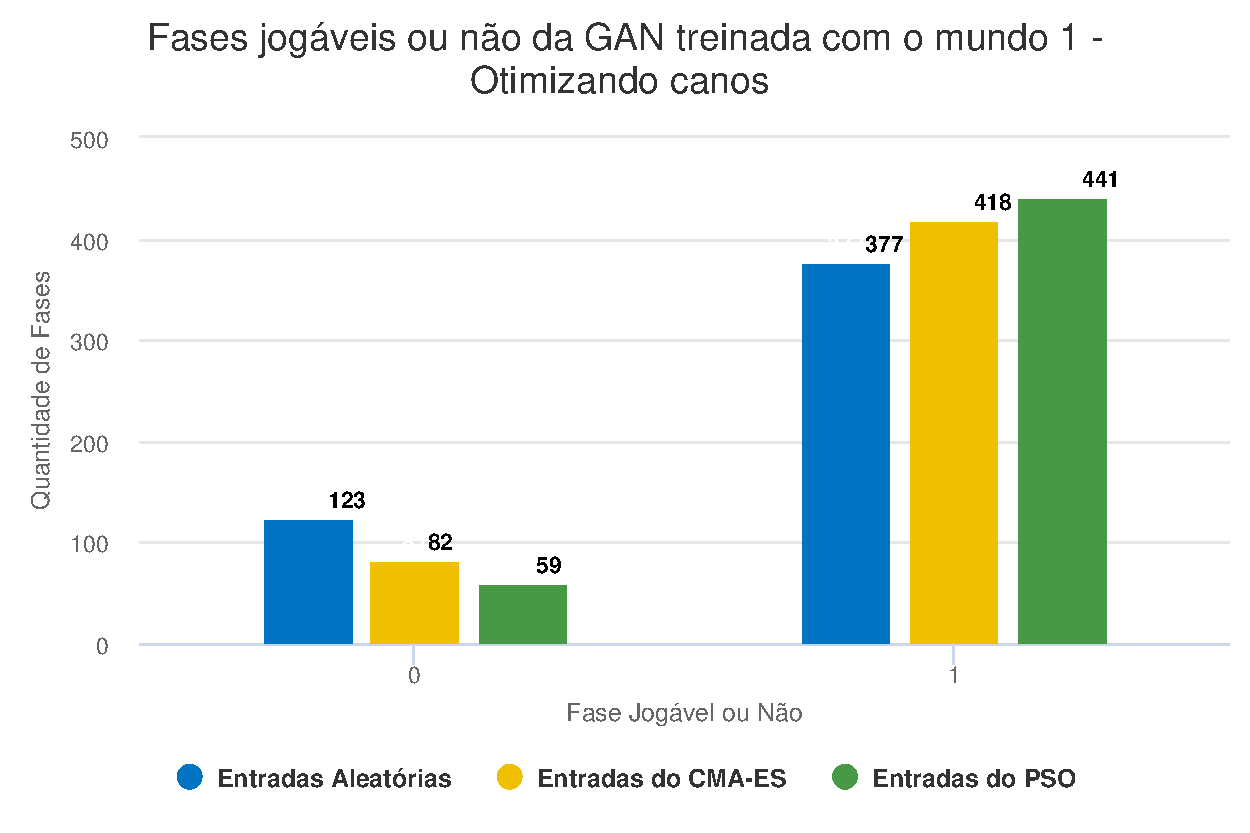
\includegraphics[width=12cm]{plots_canos/plot_wins_world_1.pdf}
\caption{Jogabilidade do Mundo 1}
\label{fig:0}
\end{figure}

Jogabilidade Mundo 2:

\begin{figure}[!htb]
\centering
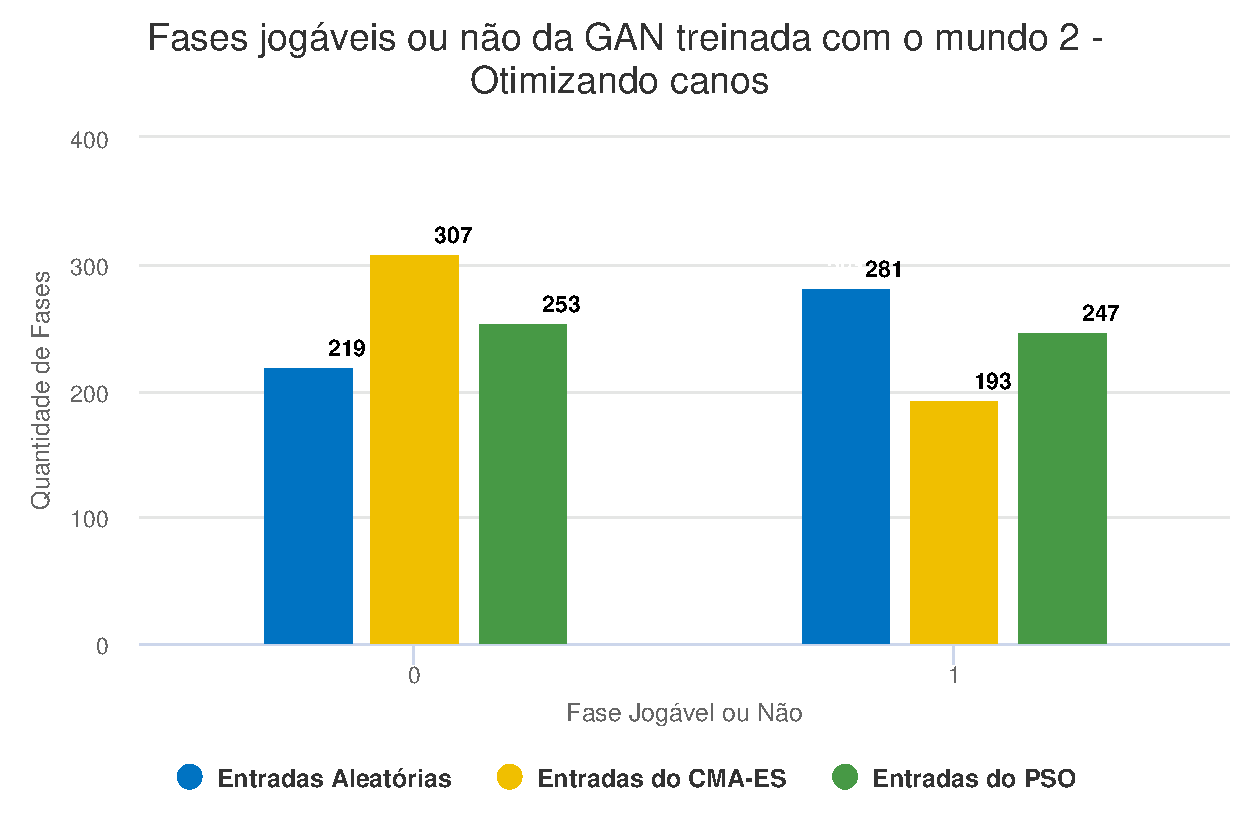
\includegraphics[width=12cm]{plots_canos/plot_wins_world_2.pdf}
\caption{Jogabilidade do Mundo 2}
\label{fig:1}
\end{figure}

Mundo 3:
\begin{figure}[!htb]
\centering
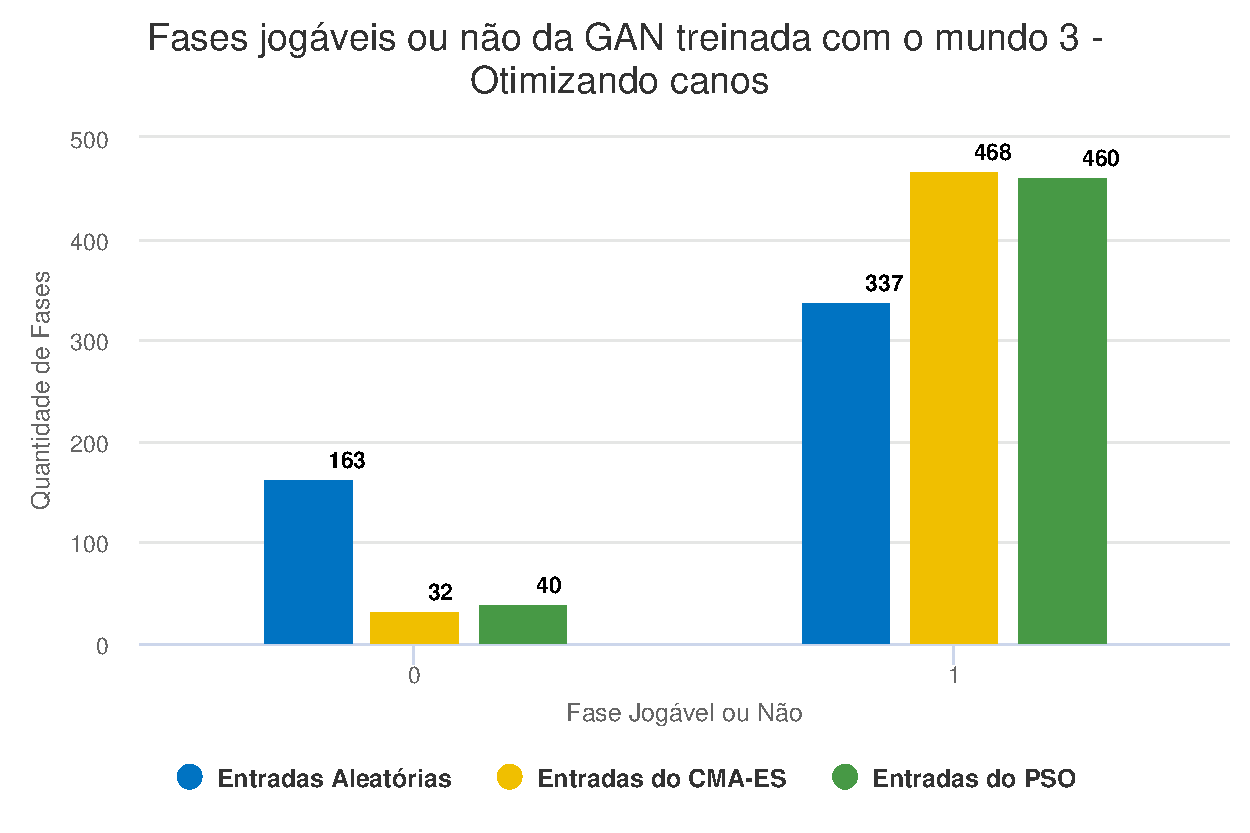
\includegraphics[width=12cm]{plots_canos/plot_wins_world_3.pdf}
\caption{Jogabilidade do Mundo 3}
\label{fig:2}
\end{figure}

Mundo 4:
\begin{figure}[!htb]
\centering
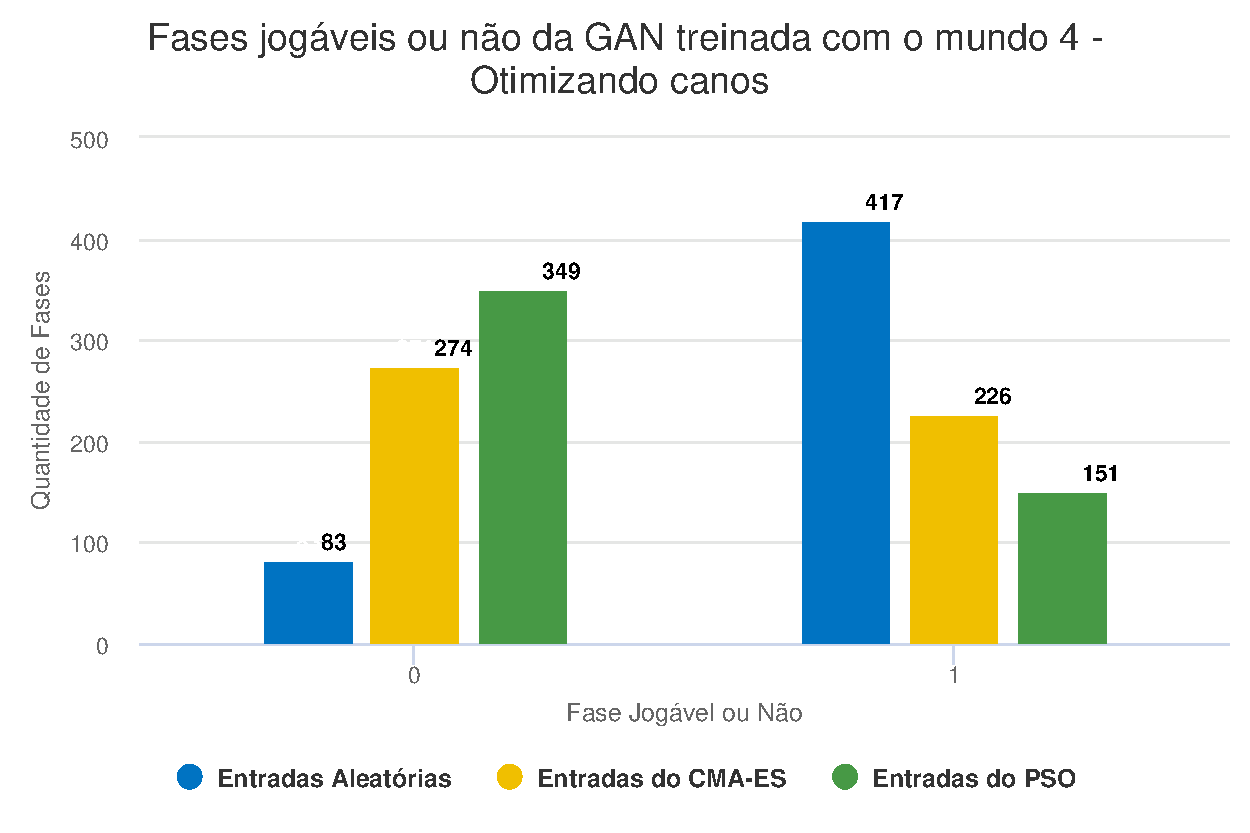
\includegraphics[width=12cm]{plots_canos/plot_wins_world_4.pdf}
\caption{Jogabilidade do Mundo 4}
\label{fig:3}
\end{figure}

Mundo 5:

\begin{figure}[!htb]
\centering
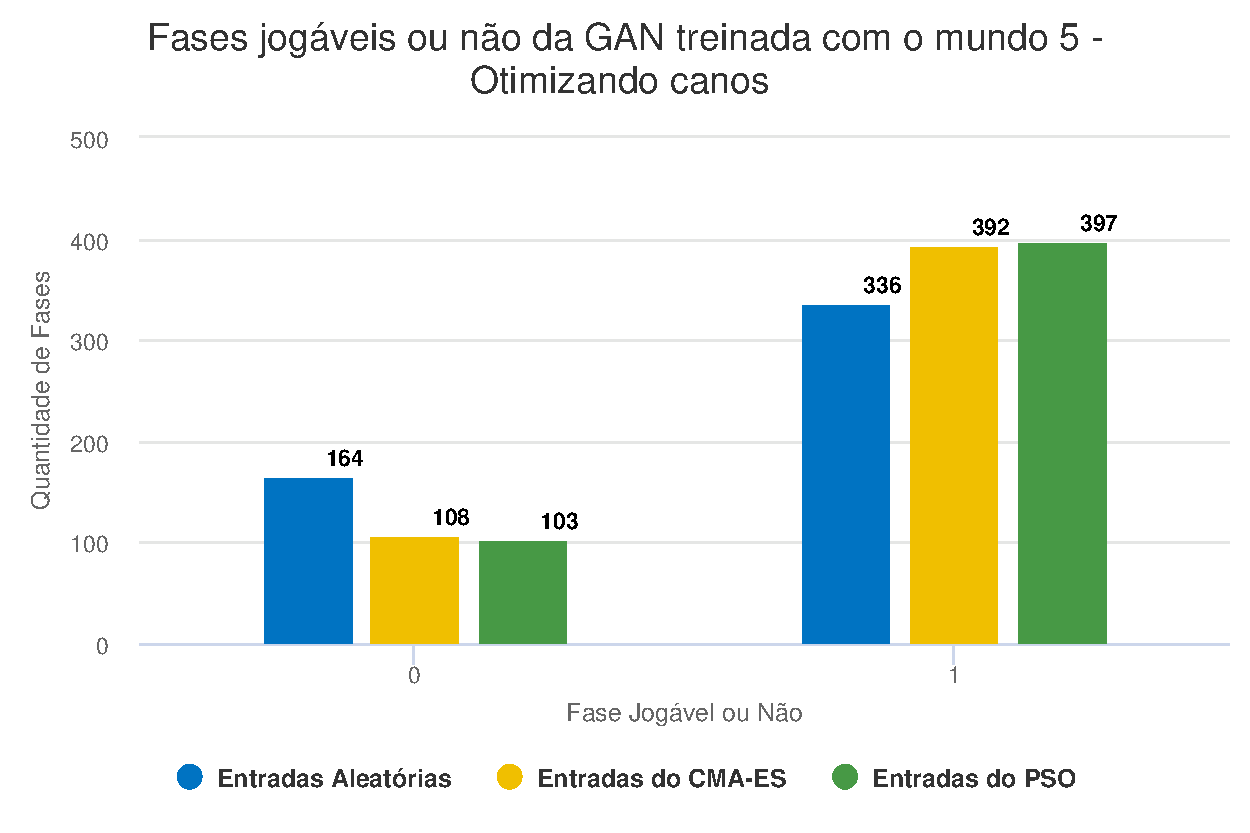
\includegraphics[width=12cm]{plots_canos/plot_wins_world_5.pdf}
\caption{Jogabilidade do Mundo 5}
\label{fig:4}
\end{figure}

Mundo 6:
\begin{figure}[!htb]
\centering
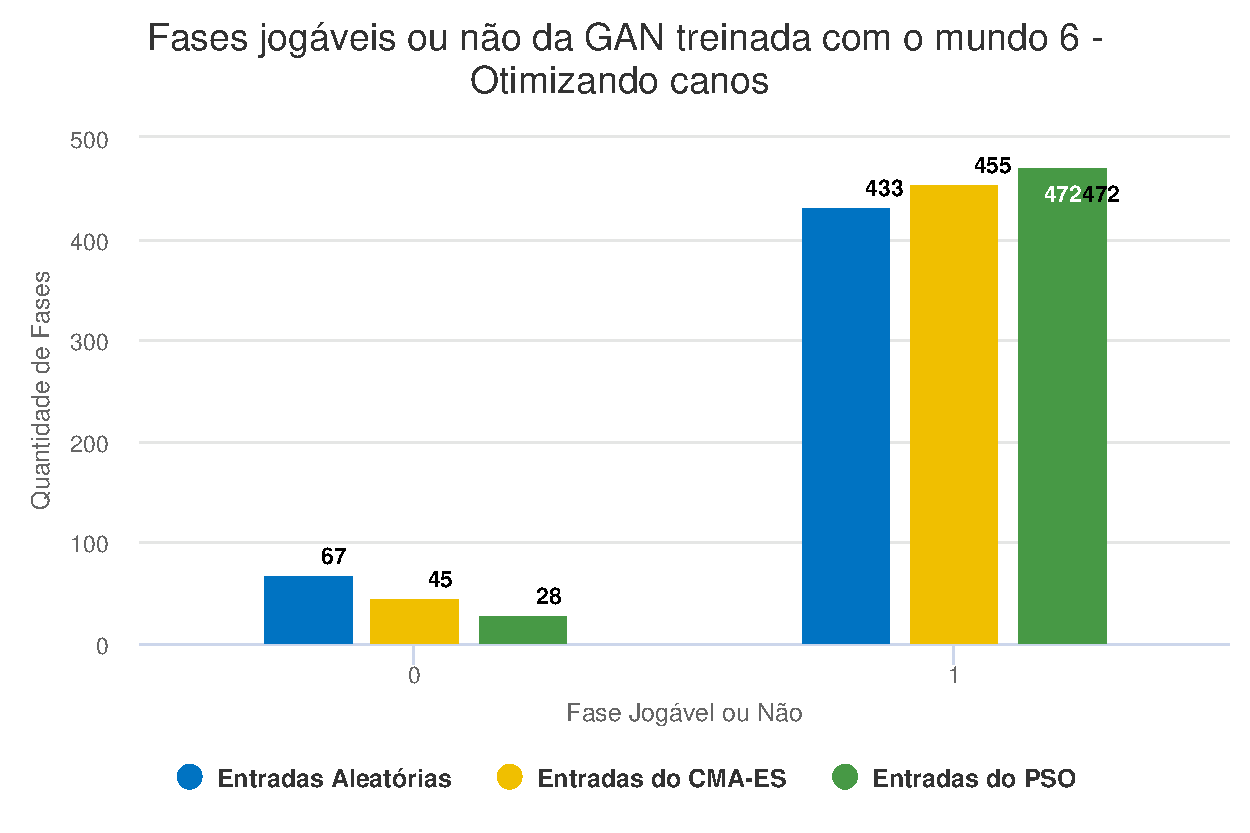
\includegraphics[width=12cm]{plots_canos/plot_wins_world_6.pdf}
\caption{Jogabilidade do Mundo 6}
\label{fig:5}
\end{figure}

Mundo 7:
\begin{figure}[!htb]
\centering
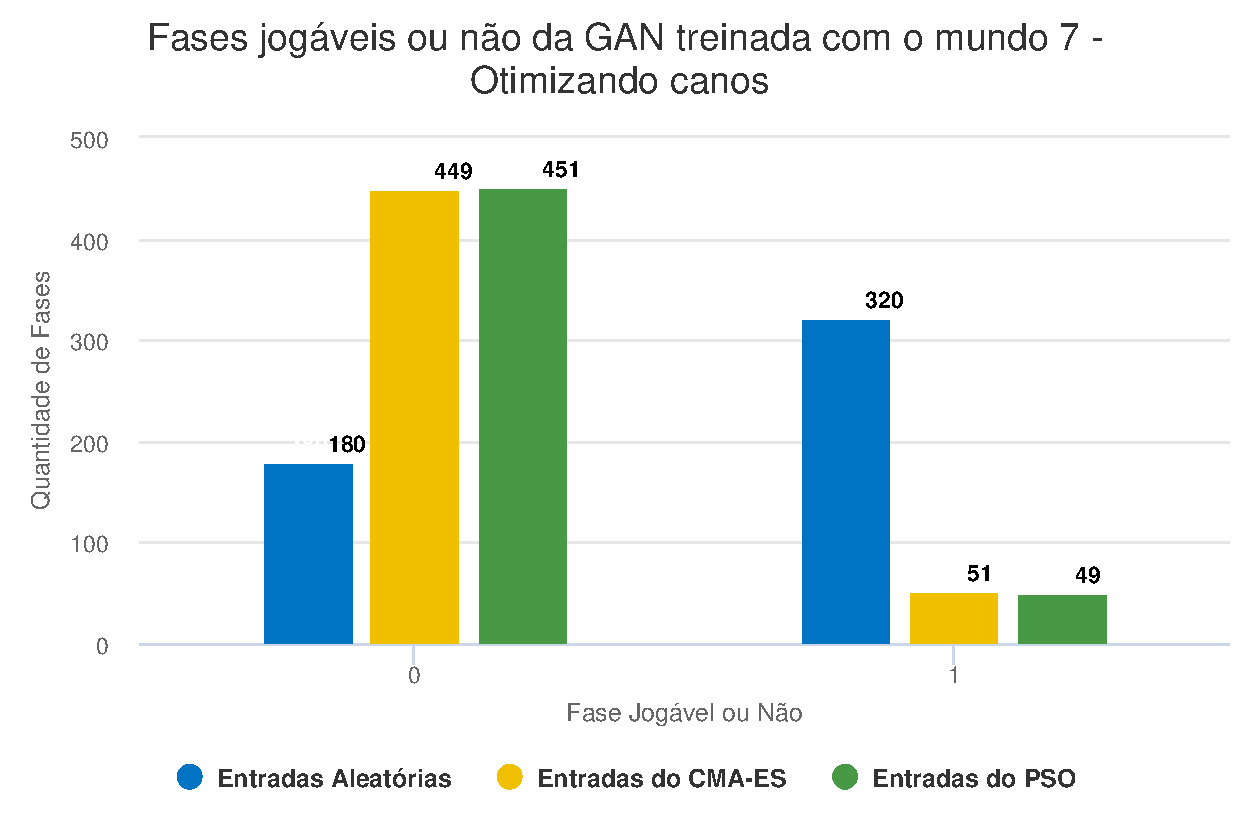
\includegraphics[width=12cm]{plots_canos/plot_wins_world_7.pdf}
\caption{Jogabilidade do Mundo 7}
\label{fig:6}
\end{figure}

Mundo 8:
\begin{figure}[!htb]
\centering
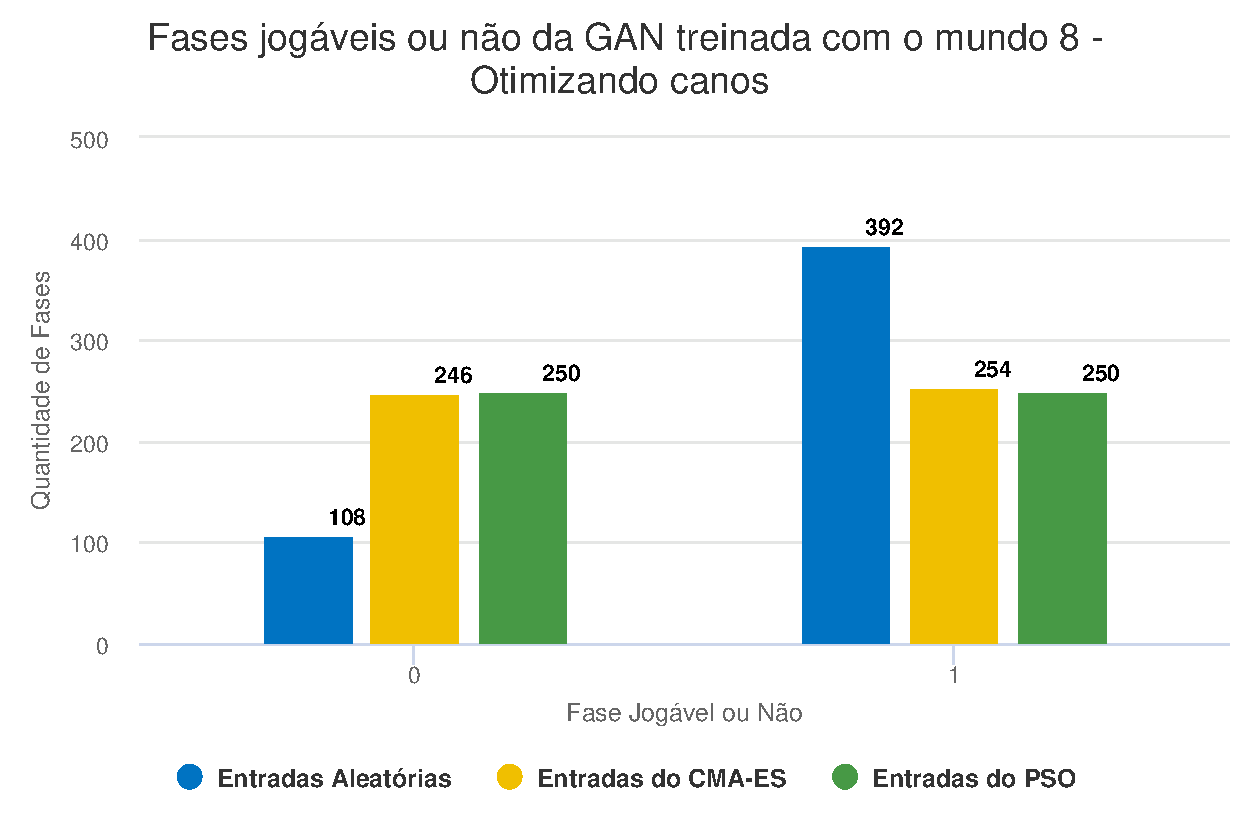
\includegraphics[width=12cm]{plots_canos/plot_wins_world_8.pdf}
\caption{Jogabilidade do Mundo 8}
\label{fig:7}
\end{figure}

\section{Jogabilidade Maximizando Inimigos}


Mundo 1:
\begin{figure}[!htb]
\centering

\includegraphics[width=12cm]{plots_inimigos/plot_wins_world_1.pdf}
\caption{Jogabilidade do Mundo 1}
\label{fig:0c}
\end{figure}

Jogabilidade Mundo 2:

\begin{figure}[!htb]
\centering

\includegraphics[width=12cm]{plots_inimigos/plot_wins_world_2.pdf}
\caption{Jogabilidade do Mundo 2}
\label{fig:1c}
\end{figure}

Mundo 3:
\begin{figure}[!htb]
\centering

\includegraphics[width=12cm]{plots_inimigos/plot_wins_world_3.pdf}
\caption{Jogabilidade do Mundo 3}
\label{fig:2c}
\end{figure}

Mundo 4:
\begin{figure}[!htb]
\centering

\includegraphics[width=12cm]{plots_inimigos/plot_wins_world_4.pdf}
\caption{Jogabilidade do Mundo 4}
\label{fig:3c}
\end{figure}

Mundo 5:

\begin{figure}[!htb]
\centering

\includegraphics[width=12cm]{plots_inimigos/plot_wins_world_5.pdf}
\caption{Jogabilidade do Mundo 5}
\label{fig:4c}
\end{figure}

Mundo 6:
\begin{figure}[!htb]
\centering

\includegraphics[width=12cm]{plots_inimigos/plot_wins_world_6.pdf}
\caption{Jogabilidade do Mundo 6}
\label{fig:5c}
\end{figure}

Mundo 7:
\begin{figure}[!htb]
\centering

\includegraphics[width=12cm]{plots_inimigos/plot_wins_world_7.pdf}
\caption{Jogabilidade do Mundo 7}
\label{fig:6c}
\end{figure}

Mundo 8:
\begin{figure}[!htb]
\centering

\includegraphics[width=12cm]{plots_inimigos/plot_wins_world_8.pdf}
\caption{Jogabilidade do Mundo 8}
\label{fig:7c}
\end{figure}

\section{Tabela De Valores Otimizando Canos}

Tabela de valores otimizando canos:
\begin{figure}[!htb]
\centering
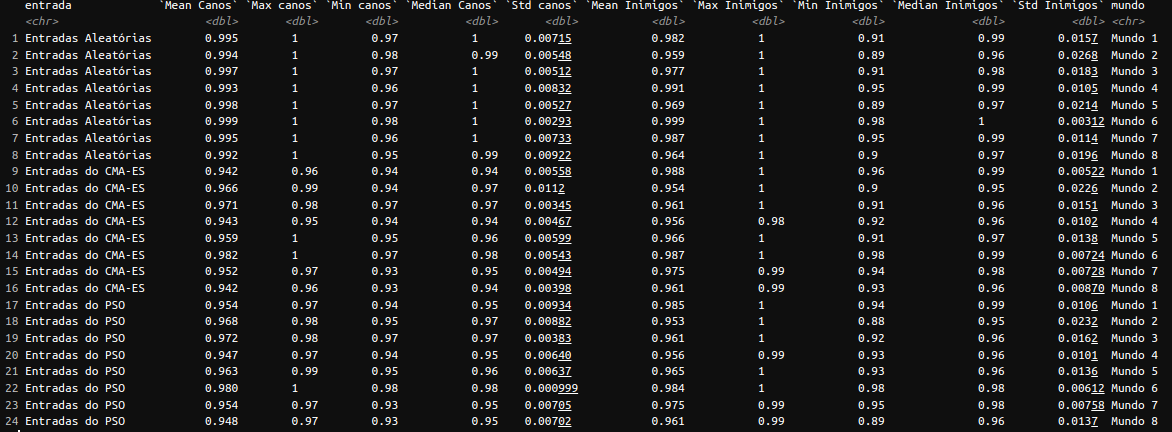
\includegraphics[width=12cm]{tabelas_otm/TABELA_OTM_CANOS.png}
\caption{Tabela Maximizando canos}
\label{fig:TO}
\end{figure}

\section{Tabela de Valores Otimizando Inimigos}

Tabela:
\begin{figure}[!htb]
\centering
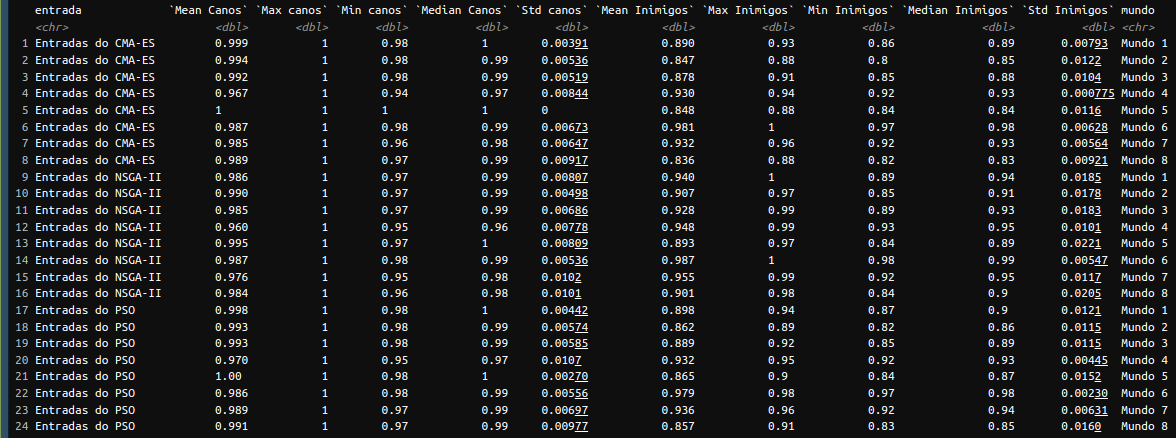
\includegraphics[width=12cm]{tabelas_otm/TABELA_OTM_INIMIGOS.png}
\caption{Tabela Inimigos}
\label{fig:TI}
\end{figure}

\section{Classificação de Padrões}


